\documentclass{article}
\usepackage{blindtext}
% \usepackage[a4paper, total={6in, 8in}]{geometry}

\usepackage{geometry}
 \geometry{
 a4paper,
 total={170mm,257mm},
 left=20mm,
 top=20mm,
 bottom=20mm
 }

\usepackage{wrapfig}
\usepackage{graphicx}
\usepackage{mathtext}
\usepackage{amsmath}
\usepackage{siunitx} % Required for alignment
\usepackage{subfigure}
\usepackage{multirow}
\usepackage{booktabs}
\usepackage{rotating}

\usepackage[T1,T2A]{fontenc}
\usepackage[russian]{babel}
\usepackage{caption}

\graphicspath{{pictures/}}


\title{\begin{center}Лабораторная работа №2.3.1\end{center}
Получение и измерение вакуума}
\author{Гёлецян А.Г.}
\date{\today}

\begin{document}
    \pagenumbering{gobble}
    \maketitle
    \newpage
    \pagenumbering{arabic}

    \textbf{Цель работы:} 1) измеренеи объёмов форвакуумной и высоковакуумной частей установки; 2) определение скорости откачки системы в стационарном режиме, а также по ухудшению и по улучшению вакуума.

    \textbf{В работе используются:} вакуумная установка с манометрами: масляным, термопарным и ионизационным.

    \section{Экспериментальная установка}

    \begin{figure}[h]
        \center{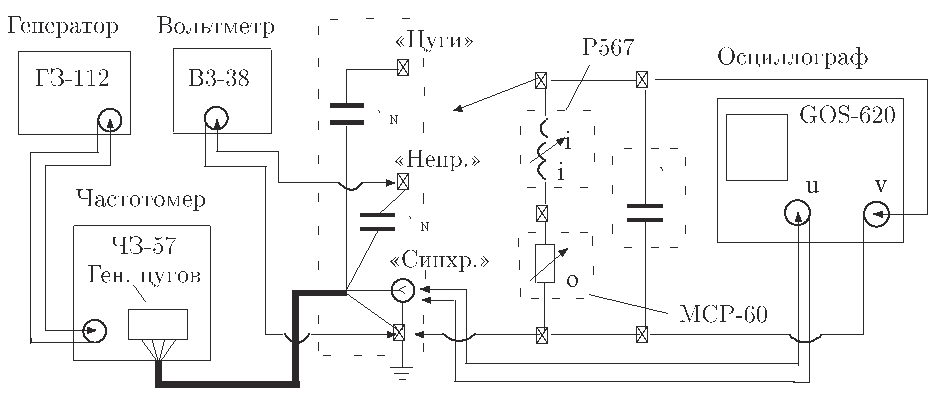
\includegraphics[width=0.8\textwidth]{ustanovka}}
        \caption{Схема экспериментальной установки.}
        \label{ris:ustanovka}
    \end{figure}

    \paragraph{}
    Установка изготовлена из стекла и состоит из форвакуумного баллона (ФБ), высоковакуумного диффузионного насоса (ВН), высоковакуумного баллона (ВБ), масляного (М) и ионизационного (И) манометров, термопарных манометров ($М_1$ и $М_2$), форвакуумного насоса (ФН) и соединительных кранов (Рис. \ref{ris:ustanovka}). Кроме того, в состав установки входят: вариатор (автотрансформатор с регулируемым выходным напряжением), или реостат и амперметр для регулирования тока нагревателя диффузионного насоса.

    \paragraph{Маслянный манометр:}
    Представляет собой U-образную трубку, до половины наполненную вязким маслом, обладающим весьма низким давлением насыщенных паров. Так как плотность масла мала, $\rho = 0,885 г/см^3$ , то при помощи манометра можно измерить только небольшие разности давлений (до нескольких торр). Во время откачки и заполнения установки атмосферным воздухом кран $К_4$ соединяющий оба колена манометра, должен быть открыт во избежание выброса масла и загрязнения установки. Кран $К_4$ закрывается только при измерении давления U-образным манометром.


    \newpage

    \paragraph{Термопарный манометр:}
    Чувствительным элементом манометра является термопара, заключенная в стеклянный баллон. Устройство термопары поясненона (Рис. \ref{ris:termoparni_monometr}). По нити накала НН пропускается ток постоянной величины. Термопара ТТ присоединяется к милливольтметру, показания которого определяются температурой нити накала и зависят от отдачи тепла вокружающее пространство. Потери тепла определяются теплопроводностью нити и термопары, теплопроводностью газа, переносом тепла конвективными потоками газа внутри лампы и теплоизлучением нити (инфракрасноетепловое излучение). В обычном режимелампы основную роль играет теплопроводность газа. При давлениях >1 торр теплопроводность газа, а вместе с ней и ЭДС термопары практически не зависят от давления газа, и прибор не работает. При улучшении вакуума средний свободный пробег молекул становится сравнимым с диаметром нити, теплоотвод падает и температура спая возрастает. При вакууме $~10^{-3}$ торр теплоотвод, осуществляемый газом, становится сравнимым с другими видами потерь теплаи температура нити становится практически постоянной. Градуировочная кривая термопарного манометра приведена на (Рис. \ref{ris:termopara_graduirovka}).

    \begin{figure}[h]
    \centering
    \begin{minipage}{0.3\textwidth}
        \centering
        \includegraphics[width=0.9\textwidth]{termoparni_monometr}
        \caption{Схема термопаного манометра.}
        \label{ris:termoparni_monometr}
    \end{minipage}\hfill
    \begin{minipage}{0.7\textwidth}
        \centering
        \includegraphics[width=0.9\textwidth]{termopara_graduirovka}
        \caption{Градуировочная кривая термопарного манометра.}
        \label{ris:termopara_graduirovka}
    \end{minipage}
    \end{figure}

    \newpage

    \paragraph{Ионизационный манометр:}
    Схема ионизационного манометра изображена на (Рис. \ref{ris:ionizacionni_monometr}). Он представляет собой трехэлектродную лампу. Электроны испускаются накаленным катодом и увлекаются электрическим полем к аноду, имеющему вид спирали. Проскакивая за ее витки,электроны замедляются полем коллектора и возвращаются к катоду, а от него вновь увлекаются к аноду. Прежде чем осесть на аноде, они успевают много раз пересечь пространство между катодом и коллектором. На своем пути электроны ионизуют молекулы газа. Ионы, образовавшиеся между анодом и коллектором, притяги ваются полем коллектора и определяют его ток. Ионный ток в цепи коллектора пропорционален плотности газа и поэтому может служить мерой давления. Вероятность ионизации зависит от рода газа, заполняющего лампу (а значит, и откачиваемый объем). Калибровка манометра верна, если остаточным газом является воздух. Накаленный катод ионизационного манометра перегорает, если давление в системе превышает $10^{-3}$ торр. Поэтому включать ионизационный манометр можно, только убедившись по термопарному манометру, что давление в системе не превышает $10^{-3}$ торр. При измерении нить ионизационного манометра сильно греется. При этом она сама, окружающие ее электроды и стенки стеклянного баллона могут десорбировать поглощенные ранее газы. Выделяющиеся газы изменяют давление в лампе и приводят к неверным показаниям. Поэтому перед измерениями ионизационный манометр прогревается (обезгаживается) в течение 10–15 мин. Для прогрева пропускается ток через спиральный анод лампы.

    \vspace{1cm}

    \begin{figure}[h]
        \center{\includegraphics[width=0.5\textwidth]{ionizacionni_monometr}}
        \caption{Схема ионизационного манометра.}
        \label{ris:ionizacionni_monometr}
    \end{figure}

    \newpage

    \paragraph{Диффузионный насос:}
    Откачивающее действие диффузионногонасоса основано на диффузии (внедрении) молекул разреженного воздуха в струю паров масла. Попавшие в струю молекулы газа увлекаются ею и уже не возвращаются назад. Устройство одной ступени масляного диффузионного насоса схематически показано на (Рис. \ref{ris:diffuzionni_nasos}) (в лабораторной установке используется несколько откачивающих ступеней). Масло, налитое в сосуд А, подогревается электрической печкой. Пары масла поднимаются по трубе Б и вырываются из сопла В. Струя паров увлекает молекулы газа,которые поступают из откачиваемого сосуда через трубку ВВ. Дальше смесь попадает в вертикальную трубу Г. Здесь масло осаждаетсяна стенках трубы и маслосборников и стекает вниз, а оставшийся газчерез трубу ФВ откачивается форвакуумным насосом. Диффузионный насос работает наиболее эффективно при давлении, когда длинасвободного пробега молекул воздуха примерно равна ширине кольцевого зазора между соплом В и стенками трубы ВВ. В этом случае пары масла увлекают молекулы воздуха из всего сечения зазора. Давление насыщенных паров масла при рабочей температуре, создаваемой обогревателем сосуда А, много больше $5\cdot10^{-2}$ торр. Именно поэтому пары масла создают плотную струю, которая и увлекаетс собой молекулы газа. Если диффузионный насос включить при давлении, сравнимом с давлением насыщенного пара масла, то последнее никакой струи не создаст и масло будет просто окисляться и угорать.

    Диффузионный насос, используемый в нашей установке, имеет две ступени и соответственно два сопла (Рис. \ref{ris:nasos_irl}). Одно сопло вертикальное (первая ступень), второе сопло горизонтальное (вторая ступень). За второй ступенью имеется еще одна печь, но пар из этой печи поступает не в сопло, а по тонкой трубке подводится ближе к печке первой ступени. Эта печь осуществляет фракционирование масла. Легколетучие фракции масла, испаряясь, поступают в первую ступень, обогащая ее легколетучей фракцией масла. По этой причине плотность струи первой ступени выше и эта ступень начинает откачивать при более высоком давлении в форвакуумной части установки. Вторая ступень обогощается малолетучими фракциями. Плотность струи второй ступени меньше, но меньше и давление насыщенных паров масла в этой ступени. Соответственно в откачиваемый объем поступает меньше паров масла и его удается откачать до более высокого вакуума, чем если бы мы работали только с одной ступенью.


    \begin{figure}[h]
    \centering
    \begin{minipage}{0.35\textwidth}
        \centering
        \includegraphics[width=1\textwidth]{diffuzionni_nasos}
        \caption{Схема одной ступени диффузионного насоса.}
        \label{ris:diffuzionni_nasos}
    \end{minipage}\hfill
    \begin{minipage}{0.65\textwidth}
        \centering
        \includegraphics[width=0.9\textwidth]{nasos_irl}
        \caption{Диффузионный насос используемый в нашей работе.}
        \label{ris:nasos_irl}
    \end{minipage}
    \end{figure}


    \section{Теоретическая часть}

    \paragraph{Процесс откачки: }
    Производительность насоса определяется скоростью откачки $W$ (л/с): W — это объем газа, удаляемого из сосуда при данном давлении за единицу времени. Скорость откачки форвакуумного насоса равна емкости воздухозаборной камеры, умноженной на число оборотов в секунду.

    Обозначим через $Q_д$ количество газа, десорбирующегося с поверхности откачиваемого объема в единицу времеи, через $Q_и$ -- количество газа, проникающего в единицу времени в этот объем извне -- через течи. Будем считать, что насос обладает скоростью откачки $W$ и в то же время сам является источником газа; пусть $Q_н$ — поток газа, поступающего из насоса назад в откачиваемую систему. $Q=Q_д + Q_и + Q_н$ измеряем в единицах (моль/с). Получаем формулу
    \begin{equation*}
        -\frac{VdP}{RT}=\left(\frac{PW}{RT} - Q\right)dt
    \end{equation*}
    При предельном давлении $dP=0$ и поэтому получаем
    \begin{equation*}
        Q=\frac{P_{пр}W}{RT}
    \end{equation*}
    Подставляя получаем
    \begin{equation*}
        -VdP=W(P-P_{пр})dt
    \end{equation*}
    Интегрируем полученное ур-е и получаем
    \begin{equation}
        P-P_{пр}=(P_0 - P_{пр})\exp\left(-\frac{W}{V}t\right)
    \end{equation}
    Пренебрегая $P_{пр}$ относитеьно $P_0$
    \begin{equation}
        P=P_0\exp\left(-\frac{W}{V}t\right)
    \end{equation}
    Как видим, величина $\tau=V/W$ показывает характерное время откачки системы.

    Теперь попробуем понять чем обусловлена скорость откачки. Очевидно, скорость $W$ зависит от скорости откачки насоса $W_н$, но она так же зависит от трубопровода соединяюшего насос к откачиваемой части, т.к. если трубопровод не сможет обеспечить достаточное количество газа к входу насоса то, производительность упадет.

    \begin{figure}[h]
        \center{\includegraphics[width=0.7\textwidth]{nasos_sketch}}
        \caption{Схема насоса с трубопроводом.}
        \label{ris:nasos_sketch}
    \end{figure}
    Попробуем описать систему математически. Пусть у нас есть насос со скоростью откачки $W_н$ и трубопровод с пропускной способностью $C$. Давление в откачиваемом объеме -- $P_1$. Исследовав схему \ref{ris:nasos_sketch} получаем

    \begin{equation*}
        C(P_1 - P_2)=W_нP_2 \Rightarrow P_2=\frac{CP_1}{C+W_н} \Rightarrow WP_1=W_нP_2=\frac{CW_н}{C+W_н}P_1
    \end{equation*}
    Как видим, для результирующей скорости $W$ верно соотношение

    \begin{equation*}
        \frac{1}{W} = \frac{1}{W_н} + \frac{1}{C}
    \end{equation*}
    Обобщая это выражение для последовательно соединенных труб получаем

    \begin{equation}
        \frac{1}{W} = \frac{1}{W_н} + \frac{1}{C_1} + \frac{1}{C_2} + ...
        \label{resulting_speed}
    \end{equation}
    Заметим только что данные формулировки верны при молекулярном режиме течения, когда вязкое трение не имеет большого вклада в движение газа.

    \paragraph{Течение газа через трубу:} Для количества газa, протекающего через трубу в условиях высокого вакуума или, как говорят, в кнудсеновском режиме, справедлива формула

    \begin{equation}
        \frac{d(PV)}{dt} = \frac{4}{3}r^3 \sqrt{\frac{2\pi RT}{\mu}} \frac{P_2 - P_1}{L}
        \label{prop_spos_truba}
    \end{equation}
    где $r$ и $L$ соответственно радиус и длина трубы. Если пренебречь давлением $P_1$ у конца, обращенного к насосу, получаем формулу для пропускной способности трубы
    \begin{equation}
    C_{тр} = \frac{dV}{dt} = \frac{4}{3}\frac{r^3}{L}\sqrt{\frac{2\pi RT}{\mu}}
    \end{equation}
    Для пропускной способности отверстия (например в кранах) имеем формулу

    \begin{equation}
    C_{отв}=S\frac{\bar v}{4}
    \end{equation}

    \section{Ход работы}

    \subsection{Измерение объема высоковакуумной части}

    Открываем все краны и запускаем в систему воздух из атмосферы ($P_{атм}=99.7\cdot 10^3 Па=748торр$). Закрываем краны $К_5$ и $К_6$, тем самым заперев в кранах и в капилляре воздух объемом $V_{зап}=(50 \pm 1)см^3$. Откачиваем воздух из системы при помощи форвакуумного насоса. После откачки до давления $\sim 10^{-2} торр$ запираем кран 2 и изолируем систему от атмосферы. Закрывая кран у масляного манометра приводим его в рабочее состояние. Отсакаем высоковакуумную часть закрытием крана 3 и впускаем запертый в кране 5 воздух в форвакуумную часть установки. при этом, давление в форвакуумной части возрастает, о чем свидетельствует маслянный манометр. Измеряем давление при помощи последнего и следующим шагом открываем кран 3, соединяя высоковакуумную часть с остальной. При этом давление падает. По этим данным считаем объем высоковакуумной части пользуясь законом Бойля-Мариотта. Заметим, что здесь мы пренебрегли начальным давлением (порядка $\sim 10^{-2} торр$) т.к. оно в $\sim 1000$ раз меньше других давлении.


    \begin{equation*}
        P_{атм}V_{зап}=P_1V_{фв}=P_2(V_{фв}+V_{вв})
    \end{equation*}
    Измеренные давления
    \begin{align*}
        \Delta h_1=(28.8 \pm 0.2) см &\Rightarrow P_1=(18.8 \pm 0.1)торр \\
        \Delta h_1=(18.3 \pm 0.2) см &\Rightarrow P_1=(11.9 \pm 0.1)торр \\
    \end{align*}
    Подставляя получаем
    \begin{align}
        V_{фв} &= (1990 \pm 40)см^3\\
        V_{вв} &= (1150 \pm 60)см^3
    \end{align}

    \subsection{Получение высокого вакуума и измерение скорости откачки}
    Открываем все краны и проводим первоначальную выкачку воздуха форвакуумным насосом. После приближения к предельному давлению ($\sim 10^{-2}торр$), закрываем кран 6 и включаем диффузионный насос. Ждем пока масло закипит и начнется дальнейшая выкачка уже диффузионным насосом. По достижению давления порядка $\sim 10^{-3}торр$ включаем ионизационный манометр, которым и будем измерять давление в дальнейшем.

    Чтобы измерить скорость откачки $W$ замерим как изменяется давление в высоковакуумной части от времени. Сосгласно теории давление должно падать по правилу, где у нас $P_{пр}=1.2\cdot10^{-4}торр$
    \begin{equation}
        P-P_{пр}=(P_0 - P_{пр})\exp\left(-\frac{W}{V_{вв}}t\right)
    \end{equation}
    Логарифмируя, получаем
    \begin{equation}
        \ln(P-P_{пр})=-\frac{W}{V_{вв}}t + c
        \label{linearized}
    \end{equation}
    Аппроксимируя наши данные согласно формуле (\ref{linearized}) получим значение для $W$. Измерение проведем 2 раза. Результаты изображены на графиках \ref{ris:ccum} (данные предоставлены в таблице \ref{plot_data}). Учитывая что погрешности логарифмов растут со временем, и зависимость теряет характерный линейный вид, линеяная аппроксимация была сделана только для оранжевых точек. Пользуясь объемом высоковакуумной части из формулы (7) и данными аппроксимации получаем следующие значения для скорости откачки


    \begin{equation}
        W_1 = (237 \pm 14)\frac{см^3}{с}; W_2 = (241 \pm 14)\frac{см^3}{с}
        \label{W_znach}
    \end{equation}
    Как видим, значеня лежат в пределах погрешности, чего и следовало ожидать.

    Теперь определим величину потока $Q_н$. Для обшего потока имеем формулу
    \begin{equation}
        P_{пр}W = (Q^\prime + Q_н)RT
        \label{Q_nasos}
    \end{equation}
    где $Q^\prime=Q_и+Q_д$. Теперь, если по достижению предельного давления закрыть кран 3, то насос будет отсоиденен от высоковакуумной части, и уравнение описывающее давление от времени примет вид

    \begin{equation*}
        V_{вв}dP = QRTdt
    \end{equation*}
    интегрируя которую получим
    \begin{equation}
        P = \frac{QRT}{V_{вв}}t + c
    \end{equation}
    Измерив зависимость давления от времени и аппроксимируя данные прямой можно получить $Q$. Графики приведены на рисунке \ref{ris:cccnum}. Отсюда получаем
    \begin{equation}
        Q_1RT=(97 \pm 6)\cdot 10^{-4}торр\cdotсм^3с^{-1};Q_2RT=(94 \pm 5)\cdot 10^{-4}торр\cdotсм^3с^{-1}
    \end{equation}
    Опять же, значения совпадают в пределах погрешности, как и ожидалось. Теперь, используя значения $W_1, W_2, Q_1, Q_2$ по формуле (\ref{Q_nasos}) считаем значение $Q_{н}$
    \begin{equation}
        Q_н=\frac{(1.9 \pm 0.3)\cdot 10^{-2}торр\frac{см^3}{с}}{RT}=(1.03 \pm 0.16)\cdot10^{-9}\frac{моль}{с}
    \end{equation}


    \begin{figure}[h]
        \centerline{\includegraphics[width=0.9\textwidth]{ccum_1}}
    \end{figure}
    \begin{figure}[h]
        \centerline{\includegraphics[width=0.9\textwidth]{ccum_2}}
        \caption{Линеаризованные графики улучшения вакуума.}
        \label{ris:ccum}
    \end{figure}

    \newpage

    \subsection{Измерение скорости откачки путем создания исскуственной течи}
    Открывая краны 5 и 6 мы создаем исскуственную течь через каппиляр. Измеряя изменение давления при создании течи можно посчитать производительность насоса. Опишем данную мысль математически. Обозначим $P_{вв}$ -- давление в высоковакуумной части, а $P_{фв}$ -- давление в форвакуумной части. До открытия каппиляра
    \begin{equation}
        \frac{P_{пр}W}{RT} = Q
    \end{equation}
    а после открытия
    \begin{equation}
        \frac{P_{уст}W}{RT} = Q + Q_{кап}
    \end{equation}
    где $P_{уст}$ -- установившееся давление после открытия каппиляра, а $C_{кап}$ -- пропускная способность каппиляра, которую считаем по формуле (\ref{prop_spos_truba}). В нашей установке

    \begin{align*}
        P_{пр}&=(1.2 \pm 0.1)\cdot10^{-4}торр\\
        P_{уст}&=(1.7 \pm 0.1)\cdot10^{-4}торр\\
        P_{фв}&=(2.3 \pm 0.1)\cdot 10^{-2}торр\\
        r&=0.4мм\\
        L&=10см\\
        T&=295К\\
    \end{align*}
    Подставляя числа получаем
    \begin{equation}
        Q_{кап}=\frac{4}{3}r^3\sqrt{\frac{2\pi RT}{\mu}}\frac{P_{фв} - P_{уст}}{LRT}=(7.7 \pm 0.3) \cdot 10^{-11} \frac{моль}{с}
    \end{equation}
    А для $W$ получаем
    \begin{equation}
    W=\frac{4}{3}\frac{r}{L}\sqrt{\frac{2\pi RT}{\mu}}r^2\frac{P_{фв} - P_{уст}}{P_{уст} - P_{пр}}=(286 \pm 80)\frac{см^3}{с}
    \end{equation}


    \section{Выводы}
    В ходе работы было измерено скорость откачки диффузионного насоса двумя способами
    \begin{equation}
        W_{ухудшение\  вакуума} = (239 \pm 14)\frac{см^3}{с}; W_{искуственная\  течь} = (286 \pm 80)\frac{см^3}{с}
    \end{equation}
    Значения совпадают в пределах погрешности. Погрешность значения измеренной методом создания исскуственной течи большая в связи с наличием разности двух близких величин в формуле подсчета($P_{уст} - P_{пр}$).

    Во время работы так же было проверенно справедливость отношения
    \begin{equation*}
        P-P_{пр}=(P_0 - P_{пр})\exp\left(-\frac{W}{V}t\right)
    \end{equation*}
    при откачке воздуха и отношения
    \begin{equation*}
        P = \frac{QRT}{V_{вв}}t + c
    \end{equation*}
    описывающее рост давления при отключении насоса от системы.

    \vspace{1cm}

    \begin{table}[!h]
    \begin{center}
    \begin{tabular}{rr|rr|rr|rr}
    \toprule
    \multicolumn{2}{c|}{Улучшение 1} & \multicolumn{2}{c|}{Улучшение 2} & \multicolumn{2}{c|}{Ухудшение 1} & \multicolumn{2}{c}{Ухудшение 2}\\
    $t, с$ &  $P, 10^{-4}торр$ & $t, с$ &  $P, 10^{-4}торр$ & $t, с$ &  $P, 10^{-4}торр$ & $t, с$ &  $P, 10^{-4}торр$\\
    \midrule
     0.0 &  7.4 &  0.0 &  7.2 &  0.0 & 1.7 &  0.0 & 1.6 \\
     0.5 &  7.3 &  0.5 &  7.0 &  1.5 & 1.8 &  1.0 & 1.7 \\
     1.0 &  7.2 &  1.0 &  6.7 &  2.5 & 1.9 &  2.0 & 1.8 \\
     1.5 &  7.0 &  1.5 &  6.3 &  3.5 & 2.0 &  3.0 & 1.9 \\
     2.0 &  6.8 &  2.0 &  5.9 &  4.5 & 2.1 &  4.5 & 2.0 \\\hline
     2.5 &  6.6 &  2.5 &  5.5 &  5.5 & 2.2 &  5.5 & 2.1 \\
     3.0 &  6.2 &  3.0 &  5.1 &  6.5 & 2.3 &  6.5 & 2.2 \\
     3.5 &  5.9 &  3.5 &  4.7 &  7.5 & 2.4 &  7.5 & 2.3 \\
     4.0 &  5.5 &  4.0 &  4.3 &  8.5 & 2.5 &  8.5 & 2.4 \\
     4.5 &  5.1 &  4.5 &  4.0 &  9.5 & 2.6 &  9.5 & 2.5 \\\hline
     5.0 &  4.7 &  5.0 &  3.7 & 10.5 & 2.7 & 11.0 & 2.6 \\
     5.5 &  4.3 &  5.5 &  3.4 & 12.0 & 2.8 & 12.0 & 2.7 \\
     6.0 &  4.0 &  6.0 &  3.2 & 13.0 & 2.9 & 13.0 & 2.8 \\
     6.5 &  3.6 &  6.5 &  3.0 & 14.0 & 3.0 & 14.0 & 2.9 \\
     7.0 &  3.4 &  7.0 &  2.8 & 15.0 & 3.1 & 15.5 & 3.0 \\\hline
     7.5 &  3.1 &  7.5 &  2.6 & 16.0 & 3.2 & 16.5 & 3.1 \\
     8.0 &  2.9 &  8.0 &  2.5 & 17.0 & 3.3 & 18.0 & 3.2 \\
     8.5 &  2.8 &  8.5 &  2.4 & 18.5 & 3.4 & 19.0 & 3.3 \\
     9.0 &  2.6 &  9.0 &  2.3 & 19.5 & 3.5 & 20.0 & 3.4 \\
     9.5 &  2.5 &  9.5 &  2.2 & 20.5 & 3.6 & 21.5 & 3.5 \\\hline
    10.0 &  2.4 & 10.0 &  2.1 & 21.5 & 3.7 & 22.5 & 3.6 \\
    10.5 &  2.3 & 11.0 &  2.0 & 23.0 & 3.8 & 24.0 & 3.7 \\
    11.0 &  2.2 & 12.0 &  1.9 & 24.0 & 3.9 & 25.0 & 3.8 \\
    11.5 &  2.1 & 13.0 &  1.8 & 25.5 & 4.0 & 26.5 & 3.9 \\
    12.0 &  2.0 & 13.5 &  1.7 & 26.5 & 4.1 & 27.5 & 4.0 \\\hline
    13.0 &  1.9 & 19.0 &  1.5 & 28.5 & 4.3 & 30.0 & 4.2 \\
    14.0 &  1.8 & 35.5 &  1.3 & 31.0 & 4.5 & 33.0 & 4.4 \\
    15.0 &  1.7 &      &      & 34.0 & 4.7 & 35.5 & 4.6 \\
    18.0 &  1.6 &      &      & 43.0 & 5.3 & 43.5 & 5.2 \\
    21.5 &  1.5 &      &      & 53.5 & 6.0 & 53.0 & 5.9 \\
    28.5 &  1.4 &      &      &      &     &      &     \\
    \bottomrule
    \end{tabular}
    \end{center}
    \caption{Данные для построения графиков}
    \label{plot_data}
    \end{table}


    \begin{figure}[h]
        \centerline{\includegraphics[width=0.9\textwidth]{cccnum_1}}
        \centerline{\includegraphics[width=0.9\textwidth]{cccnum_2}}
        \caption{Графики ухудшения вакуума.}
        \label{ris:cccnum}
    \end{figure}

\end{document}



